\documentclass[a4paper,10pt,titlepage]{article}
% PREUMBULUM
\usepackage[utf8]{inputenc}
\usepackage[T1]{fontenc}

\usepackage{a4wide} 
\usepackage{times}

\usepackage[magyar,english]{babel}

% Forráskódoknak:
\usepackage{listings}

% Tartalomjegyzék:
\usepackage{tocbibind}

\usepackage[usenames,dvipsnames]{color}

% Hogy legyen képünk:
\usepackage{graphicx}

%###############################################################################
\newcommand{\szerzo}{\input{szerzok.inc}}
\newcommand{\cim}{Hallgatói előrehaladás támogató ''badge'' rendszer \\ Telepítési dokumentáció}
\newcommand{\cimmeta}{Hallgatói előrehaladás támogató ''badge'' rendszer - Telepítési dokumentáció}
\newcommand{\targy}{}
\newcommand{\kulcsszavak}{}

\usepackage{hyperref}
\hypersetup{
    unicode=true,
    colorlinks=true,
    linkcolor=RoyalBlue,
    citecolor=RoyalBlue,
    filecolor=RoyalBlue,
    urlcolor=RoyalBlue,
    pdftitle={\cimmeta},        % title
    pdfauthor={\szerzo},    % author
    pdfsubject={\targy}, % subject of the document
    pdfkeywords={\kulcsszavak},    % list of keywords
}

\usepackage{url}

% Táblázatoknak:
\usepackage{colortbl}

% Ha kell matek:
\usepackage{amssymb,amsmath}

\usepackage{verbatim} % Hogy lehessen blokkkommentezni

% Egymás melleti képekhez:
\usepackage{subfig}

\setlength{\parindent}{12pt} % magyar nyelvű dokumentumokban jellemző
\setlength{\parskip}{0pt}    % magyar nyelvű dokumentumokban jellemző

\usepackage{setspace}  % Ettol a tablazatok, abrak, labjegyzetek maradnak 1-es sorkozzel!

%###########################################
% Saját eszközök:
%
\definecolor{todobgszin}{rgb}{0.64,0.78,0.22}
\definecolor{todofrszin}{rgb}{0.00,0.50,0.00}

\newcommand{\angolul}[1]{\foreignlanguage{english}{#1}}

\newcommand{\todo}[1]{
    \vfill
    \begingroup % Csinálunk egy csoportot, hogy az identálás csak erre vonatkozzon
        \setlength{\parindent}{0cm} % Beállítjuk, hogy teljes szélességű legyen a dobozunk a bekezdéstől függetlenül
        \fcolorbox{todofrszin}{todobgszin}{
            \parbox{\textwidth}{
                \vskip10pt
                \leftskip10pt
                \rightskip10pt
            
                \emph{TODO: #1}
  
                \vskip10pt
            }
        }
    \endgroup
    \vfill
}

\newenvironment{sajat_itemize}
{
	\begin{itemize}
	\setlength{\itemsep}{0pt}
}
{
	\end{itemize}
}

\begin{document}
% Dokumentumtörzs

\selectlanguage{magyar}

% Címoldal:
\begin{titlepage}

\title{\cim}
\author{\szerzo}
\date{\today}

\end{titlepage}
\maketitle

% Nem akarom, hogy megjelenjen a tartalomjegyzékben a Tartalomjegyzék:
\section*{Tartalomjegyzék}
\makeatletter
\@starttoc{toc}
\makeatother

\section{A rendszer telepítéséhez és működéséhez szükséges szoftveres előkövetelmények}

Jelen dokumentáció Linux rendszerre való telepítést ír le, de Windows platform esetén sincs lényegi különbség az egyes lépések során. Feltételezzük, hogy a következő szoftverek már telepítve vannak:
\begin{sajat_itemize}
\item Python (v2.7.3) (\url{http://python.org/})
\item virtualenv csomag (v1.8.3) (\url{http://www.virtualenv.org/en/latest/})
\item a szoftver repository közvetlen eléréséhez git verziókezelő
\end{sajat_itemize}

\section{A szoftver forrásának telepítése}

Amennyiben rendelkezünk a szoftver forrását tartalmazó ZIP állománnyal, úgy azt csak tömörítsük ki a számunkra megfelelő helyre. Ha nem akkor a következő módon tudjuk letölteni a szoftver repository-jából:
\begin{verbatim}
git clone https://github.com/reedcourty/badge-aut.git
\end{verbatim}

Ezután adjuk ki a \texttt{git checkout dev} parancsot, hogy a fejlesztői ágat használjuk.

\section{Futtató környezet létrehozása}

Lépjünk be a szoftver könyvtárába:

\begin{verbatim}
user@host:~$ cd badge-aut/
user@host:~/badge-aut$
\end{verbatim}

Hozzuk létre a \textit{virtualenv} környezetet:

\begin{verbatim}
user@host:~/badge-aut$ virtualenv venv
\end{verbatim}

A következő kimenetet kell látnunk:

\begin{verbatim}
New python executable in venv/bin/python
Installing setuptools............done.
Installing pip...............done.
\end{verbatim}

Aktiváljuk a környezetet:

\begin{verbatim}
user@host:~/badge-aut$ . venv/bin/activate
\end{verbatim}

Telepítsük a Django keretrendszert és a PIL képkezelő csomagot:

\begin{verbatim}
(venv)user@host:~/badge-aut$ easy_install -U django
(venv)user@host:~/badge-aut$ easy_install -U pil
\end{verbatim}

\section{Szerverkörnyezet beállítása}

Szerkesszük a \texttt{badge\_out/badge\_out/settings.py} állományt. A
\begin{verbatim}
DEBUG = True
\end{verbatim}
sort állítsuk \texttt{False}-ra, kikapcsolva ezzel a felhasználók számára értelmetlen hibaüzeneteket. Ezután állítsuk be az adatbázis elérését. Mivel most SQLite adatbázis-kezelőt használunk, ezért nem térünk ki más megoldás ismertetésére.
A következőképpen kell kinéznie a konfigurációnak:

\begin{verbatim}
DATABASES = {
    'default': {
        'ENGINE': 'django.db.backends.sqlite3',
        'NAME': PROJECT_PATH + 'badge-out.sqlite',
        'USER': '',
        'PASSWORD': '',
        'HOST': '',
        'PORT': '',
    }
}
\end{verbatim}

Keressük meg a SECRET\_KEY-t tartalmazó sort és adjunk meg egy tetszőleges véletlen karaktersorozatot, pl.

\begin{verbatim}
SECRET_KEY = '^rf5(hq_8u83j4;.w6542664l5+%+D+R+R25p;_%-feg7-k_'
\end{verbatim}

Ezután mentsük el az állományt.

\section{Adatbázis inicializálása és adminisztrátor létrehozása}

\begin{verbatim}
(venv)user@host:~/badge-aut$ cd badge_out/
(venv)user@host:~/badge-aut/badge_out$ python manage.py syncdb
\end{verbatim}

Az utasítás hatására létrejönnek a rendszer adattáblái, majd a következő kérdést teszi fel a script:

\begin{verbatim}
You just installed Django's auth system, which means you 
don't have any superusers defined.
Would you like to create one now? (yes/no):
\end{verbatim}

Válaszoljunk \textit{yes}-szel, majd a további kérdésekre értelemszerűen válaszoljunk. Ezután létrejön egy adminisztrátor felhasználó, amivel a rendszer használhatjuk majd.

\section{A szerver elindítása}

A szerver elindítani a következő módon tudjuk:
\begin{verbatim}
(venv)user@host:~/badge-aut/badge_out$ python manage.py runserver 
    0.0.0.0:8080
\end{verbatim}

Ezután a szerver URL-jét megadva a böngészőnek, kiegészítve a \texttt{/admin} végződéssel elérhetjük a rendszer adminisztrációs felületét (\ref{fig:django_admin}.~ábra).

\begin{figure}[ht!]
\centering
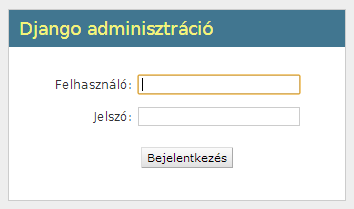
\includegraphics[width=0.50\textwidth]{figures/django_admin.png}
\caption{A rendszer adminisztrációs felületének bejelntkezési felülete \label{fig:django_admin}}
\end{figure}

\section{A rendszer használata}

A rendszerhasználatának megkezdéséhez létre kell hozni min. 1 oktató szerepet betöltő felhasználót, aki később létre tudja, hozni a célokat, feladatokat, badge-eket stb. Ezután már az oktató is be tud lépni a nyitó oldalon.

\end{document}